\documentclass[a4paper]{article}
\usepackage{booktabs}
\usepackage{geometry}
\geometry{
  top=1in,
  inner=1in,
  outer=1in,
  bottom=1in,
  headheight=3ex,
  headsep=2ex
}
\usepackage{amssymb,amsmath}
\usepackage{fontspec}
\usepackage[CJKbookmarks, colorlinks, bookmarksnumbered=true,pdfstartview=FitH,linkcolor=blue,citecolor=black]{hyperref}
\usepackage{xeCJK}
\usepackage{xltxtra,xunicode}
\usepackage{listings}
\usepackage{xcolor}
\usepackage{array}
\usepackage{float}

\lstset{basicstyle=\footnotesize\ttfamily,        % size of fonts used for the code
        columns=fullflexible,
        numbers=left,
        numberstyle=\tiny,
        keywordstyle=\color{blue},
        stringstyle=\color[rgb]{0,0.6,0},
        commentstyle=\color[cmyk]{1,0,1,0},
        frame=shadowbox,
        escapeinside=``,
        breaklines=true,
        extendedchars=false,
        xleftmargin=2em,xrightmargin=2em, aboveskip=1em,
        tabsize=4, %tab size
        showspaces=false %no space
       }

\newcommand{\tightlist}{
  \setlength{\itemsep}{0pt}\setlength{\parskip}{0pt}}

% font
\setCJKmainfont[AutoFakeBold]{文泉驿微米黑}
\setmainfont[AutoFakeBold]{Segoe UI}
\setromanfont[AutoFakeBold]{Segoe UI}
\setmonofont[Mapping={}]{Monaco}
\linespread{1.2}\selectfont
\XeTeXlinebreaklocale "zh" 
\setcounter{secnumdepth}{3}
\begin{document}
\title{\Huge Java技术\\ 最终上机报告}
\author { \vspace{12cm} \\ \LARGE 班级:  1413014  \\ \LARGE 姓名:  乔新文   \\ \LARGE 学号:14130140393} 
\date{ \vspace{4cm} 2017.5.28}

\maketitle
\clearpage

\tableofcontents

\clearpage

\section{综述}

本文档将阐述《Java技术》最终上机代码的详细设计及实现。\\

为节约篇幅,文档中对上机要求中已有的部分将不再复述,仅对总体的设计思路,要求外添加的内容和部分重要的代码做出说明。\\

本项目代码遵循GPL v2.0 协议开源,仓库地址 \url{https://github.com/starsriver/JavaHomework} \\

本次上机实验所用使用Maven3工具管理项目引用和代码,并进行自动化编译及打包。\\

编译并打包命令(项目主目录下):mvn package \\

打包好的jar文件位于项目主目录/target下,使用:java -jar HWF-0.1.jar 即可运行。\\

本次上机所有代码均在本机(Win10 10586 64位 JDK1.8)上经过测试并运行正常,其他环境下则未经测试。

\section{题目一}

\subsection{题目}

PIM - Personal Information Manager ( GUI )

\subsection{设计阐述}
    \subsubsection{总体设计}
        项目使用典型的MVC模式,分离视图,控制和数据模型。\\
        StarsRiver.MainWindows.main方法为程序入口,负责接受命令行参数并设置基本的数据模型,随后加载主View页面和对应的Controller。\\
        主View页面main.fxml初始化项目使用的视图模型并将页面中的控件与Controller中的控件定义和时间定义绑定,随后等待用户交互。\\
        当用户交互动作发生时,触发对应的事件并产生响应,由不同的交互动作和交互位置触发不同的操作修改视图模型。
        视图模型的修改引发界面内容更新,界面内容更新后继续等待下一个用户交互动作。
    \subsubsection{View}
        View部分使用JavaFX编写,包括所有呈现给用户的视觉界面,所有fxml文件位于src/main/resources/View目录下。\\
    \subsubsection{Model}
        Model部分为项目中使用的PIM数据模型和集合类型,位于src/main/StarsRiver/Model目录下。\\
    \subsubsection{Controller}
        Controller部分中使用的操作类集合,包括储存操作过程,View对应的用户交互过程,位于src/main/StarsRiver/Controller目录下。\\

\subsection{Model设计}
    Model为项目使用的自定义数据模型,包含基础的PIMEntity,PIMDate以及衍生出的PIMTodo,PIMNote,PIMContact,PIMAppointment,PIMCollection,PIMManager。\\
    
    \begin{figure}[h]
        \centering
        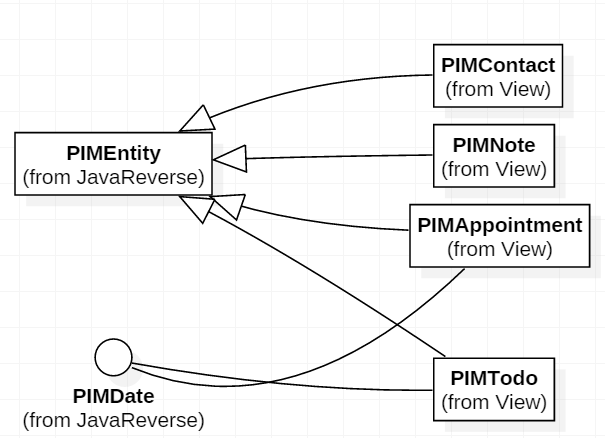
\includegraphics[width=8cm]{summe02r.PNG}\\
    \end{figure}
    Model部分已在报告2,报告3中做过详细阐述,故此处不再冗述。\\
\subsection{View设计}
    View部分呈现给用户的视觉界面,主要分为数据呈现部分和用户交互部分。\\
    \subsubsection{数据呈现部分}
        用来显示日历以及对应日期的PIMEntity内容和日期无关的PIMNote和PIMContact。\\
        显示的内容会随当前日期的变化而改变。\\
        \begin{figure}[h]
            \centering
            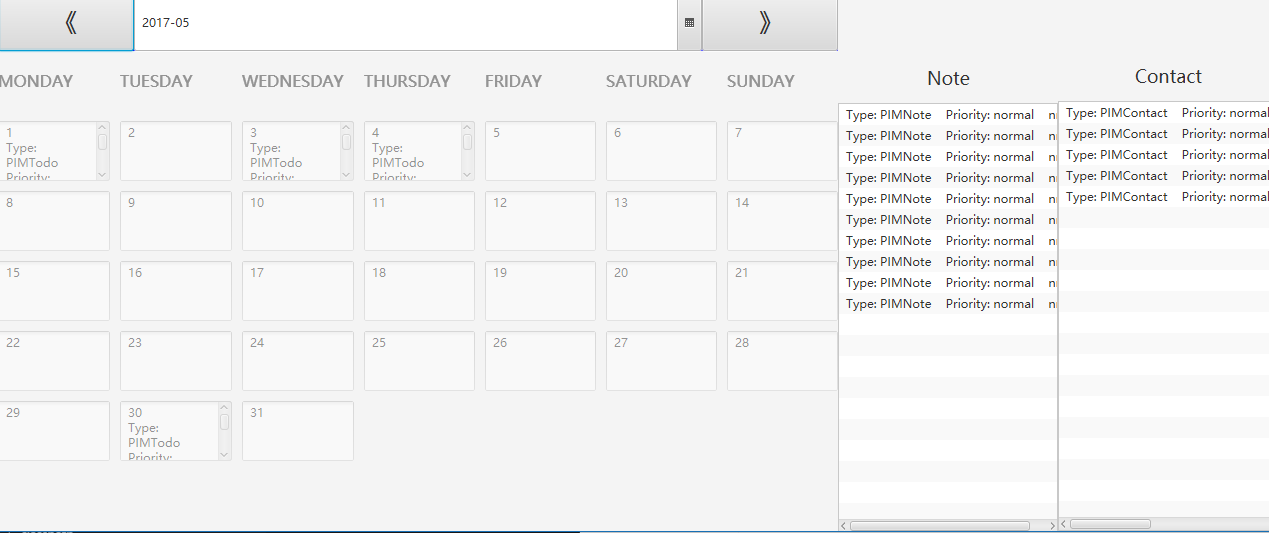
\includegraphics[width=8cm]{SYNC2.png}\\
        \end{figure}
    \subsubsection{用户交互部分}
        用来引导用户进行PIM系统的操作,包括变更日期,创建PIMEntity项目,控制数据呈现部分展示的数据和读取,储存数据。\\
        显示的内容会随当前日期的变化而改变。\\
        \begin{figure}[h]
            \centering
            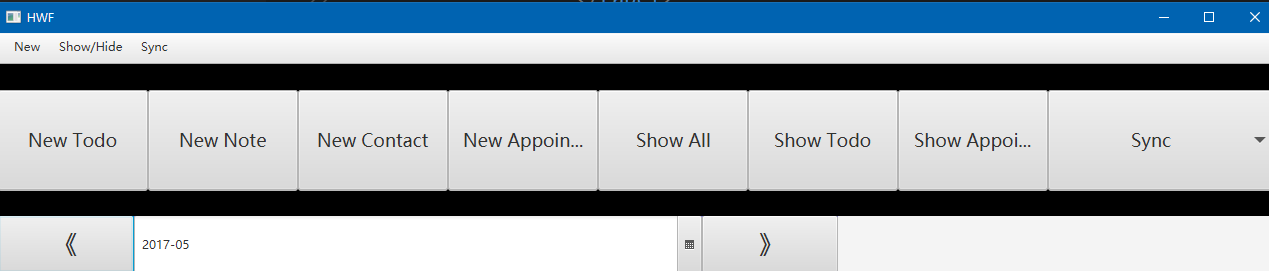
\includegraphics[width=8cm]{SYNC3.png}\\
        \end{figure}\\
        \begin{figure}[h]
            创建新的PIMEntity:\\
            \centering
            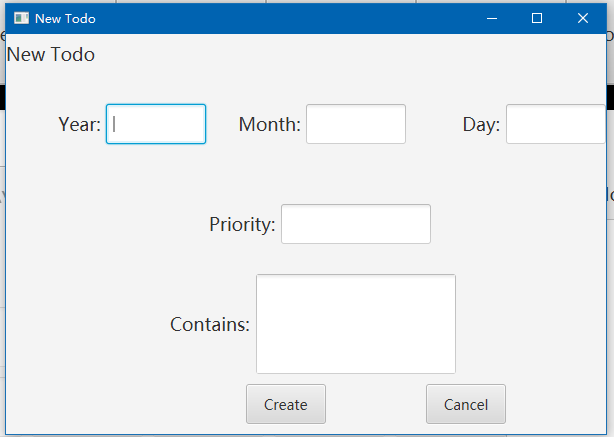
\includegraphics[width=4cm]{n1.png}
            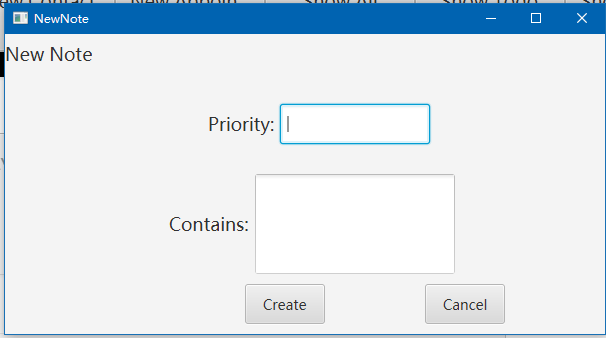
\includegraphics[width=4cm]{n2.png}\\
            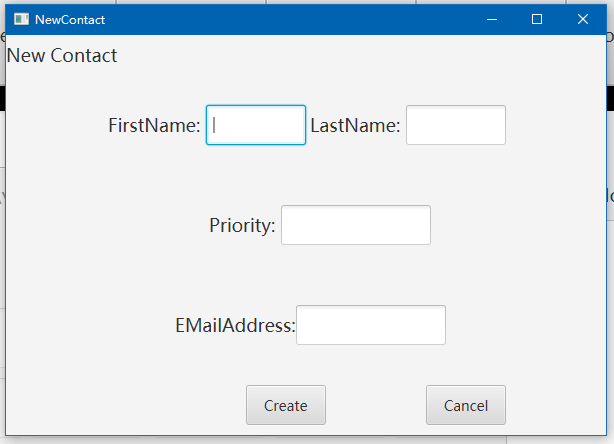
\includegraphics[width=4cm]{n3.png}
            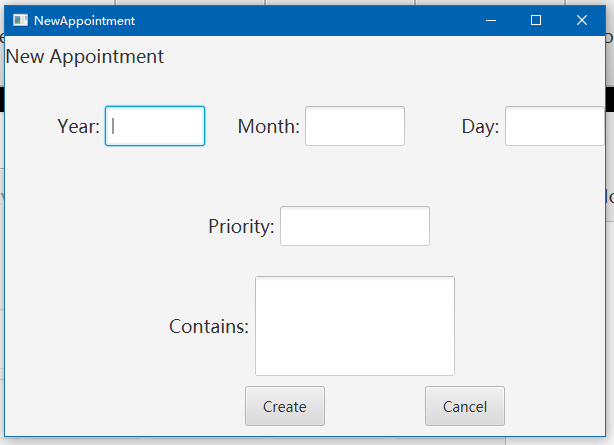
\includegraphics[width=4cm]{n4.png}\\
        \end{figure}\\
        \begin{figure}[H]
            打开,储存操作:\\
            \centering
            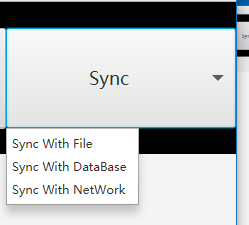
\includegraphics[width=4cm]{s.png}\\
            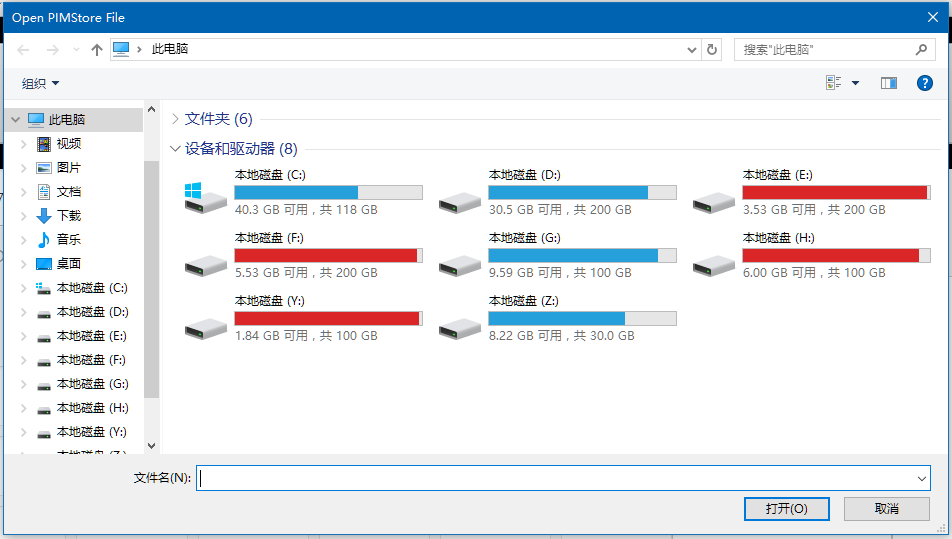
\includegraphics[width=4cm]{s12.png}
            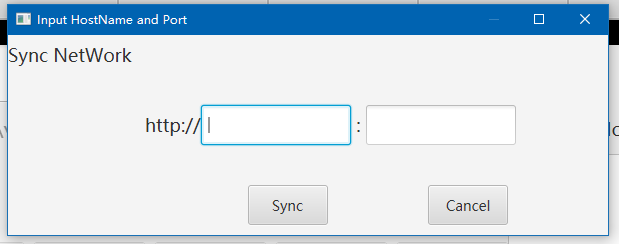
\includegraphics[width=4cm]{s3.png}\\
        \end{figure}
\subsection{Controller设计}
    Controller部分中使用的操作类集合,包括储存操作过程,View对应的用户交互过程。
    \subsubsection{储存操作过部分}
    包含对本地文件,Sqlite3数据库,远程服务器的读写操作
    \begin{figure}[h]
        \centering
        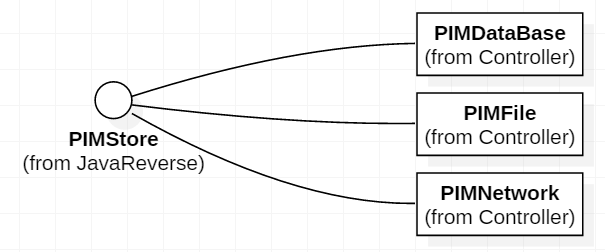
\includegraphics[width=8cm]{summe03.PNG}\\
    \end{figure}
    \subsubsection{用户交互过程部分}
        对应View中可交互控件交互过程中对应的事件响应,大致可分为数据模型操作部分,用户交互提示部分,界面内容跟新部分。\\
\subsection{部分代码}
    \subsubsection{View部分}
        与远程服务器同步数据View,提示用户输入远程服务器的地址和端口
        \begin{lstlisting}[language=xml]
<?xml version="1.0" encoding="UTF-8"?>
<?import javafx.scene.text.*?>
<?import javafx.scene.control.*?>
<?import java.lang.*?>
<?import javafx.scene.layout.*?>

<Pane maxHeight="-Infinity" maxWidth="-Infinity" minHeight="-Infinity" minWidth="-Infinity" prefHeight="200.0" prefWidth="600.0" xmlns="http://javafx.com/javafx/8" xmlns:fx="http://javafx.com/fxml/1" fx:controller="StarsRiver.Controller.SyncNetWorkController">
   <children>
      <VBox prefHeight="200.0" prefWidth="600.0">
         <children>
            <HBox prefHeight="40.0" prefWidth="600.0">
               <children>
                  <Label fx:id="Title" prefHeight="40.0" prefWidth="600.0" text="Sync NetWork">
                     <font>
                        <Font size="18.0" />
                     </font>
                  </Label>
               </children>
            </HBox>
            <HBox alignment="CENTER" prefHeight="100.0" prefWidth="600.0">
               <children>
                  <Label alignment="CENTER_RIGHT" prefHeight="80.0" prefWidth="100.0" text="http://">
                     <font>
                        <Font size="18.0" />
                     </font>
                  </Label>
                  <TextField fx:id="HostName" prefHeight="40.0" prefWidth="150.0" />
                  <Label alignment="CENTER_RIGHT" prefHeight="80.0" prefWidth="15.0" text=" : ">
                     <font>
                        <Font size="18.0" />
                     </font>
                  </Label>
                  <TextField fx:id="Port" prefHeight="40.0" prefWidth="150.0" />
               </children>
            </HBox>
            <HBox alignment="CENTER_RIGHT" prefHeight="60.0" prefWidth="600.0">
               <children>
                  <Button fx:id="Sync" mnemonicParsing="false" onAction="#Sync" prefHeight="40.0" prefWidth="80.0" text="Sync">
                     <font>
                        <Font size="14.0" />
                     </font>
                  </Button>
                  <Label prefHeight="80.0" prefWidth="100.0" />
                  <Button fx:id="Cancel" mnemonicParsing="false" onAction="#Cancel" prefHeight="40.0" prefWidth="80.0" text="Cancel">
                     <font>
                        <Font size="14.0" />
                     </font>
                  </Button>
                  <Label prefHeight="80.0" prefWidth="100.0" />
               </children>
            </HBox>
         </children>
      </VBox>
   </children>
</Pane>

        \end{lstlisting}
        \begin{figure}[H]
            视图渲染效果:\\
            \centering
            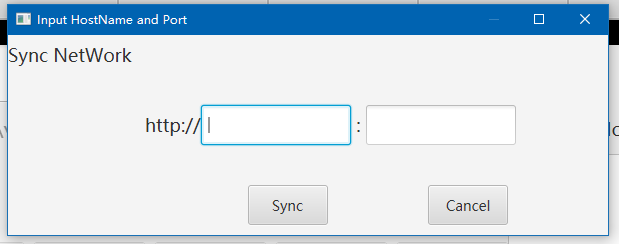
\includegraphics[width=8cm]{s3.png}\\
        \end{figure}
    \subsubsection{Model部分}
    对指定格式的字符串数组反序列化生成PIMEntity项目集合。
    \begin{lstlisting}[language=Java]
    public PIMCollection(String[] pimCollectionStrings){
        super();
        for(int i = 0; i<pimCollectionStrings.length;i++){
            try{
                switch(pimCollectionStrings[i].substring(0, 13)){
                    case "Type: PIMTodo":{
                        this.add(PIMTodo.FromString(pimCollectionStrings[i]));
                        break;
                    }
                    case "Type: PIMNote":{
                        this.add(PIMNote.FromString(pimCollectionStrings[i]));
                        break;
                    }
                    case "Type: PIMAppo":{
                        this.add(PIMAppointment.FromString(pimCollectionStrings[i]));
                        break;
                    }
                    case "Type: PIMCont":{
                        this.add(PIMContact.FromString(pimCollectionStrings[i]));
                        break;
                    }
                    default:{
                        System.out.println(pimCollectionStrings[i] + " Can't Parse");
                    }
                }
            }
            catch(IndexOutOfBoundsException e){
                System.out.println(pimCollectionStrings[i] + " Can't Parse");
                continue;
            }
        }
    }
    \end{lstlisting}

    PIMCollection 中提取与给定日期相同的PIMTodo项目和PIMAppointment项目。
    \begin{lstlisting}[language=Java]
    public PIMCollection getItemsForDate(LocalDate d){
        PIMCollection entitiesForDate = new PIMCollection();
        for(PIMEntity item:this){
            if((item instanceof PIMDate )&&((PIMDate)item).getDate().equals(d)){
                entitiesForDate.add(item);
            }
        }
        return entitiesForDate;
    }
    public HashSet<PIMEntity> getItemsForDate(Date d){
        LocalDate ld = d.toInstant().atZone(ZoneId.systemDefault()).toLocalDate();
        return getItemsForDate(ld);
    }
    \end{lstlisting}

\subsubsection{Controller部分}
    从命令行输入的参数设置数据模型并加载主页面。
    \begin{lstlisting}[language=Java]
public class MainWindows extends Application{

    public static LocalDate date;
    public static PIMCollection pimcollection;
    static{
        date = LocalDate.now();
        pimcollection = new PIMCollection();
    }

    @Override
    public void start(Stage primStage) throws Exception {
        Parent root = FXMLLoader.load(getClass().getResource("/View/main.fxml"));
        primStage.setTitle("HWF");
        primStage.setScene(new Scene(root));
        primStage.show();
    }
    public static void main(String[] args) {
        if(args.length >= 1){
            try{
                StarsRiver.MainWindows.date = LocalDate.parse(args[0],DateTimeFormatter.ofPattern("yyyy-MM-dd"));
            }
            catch(Exception e){
                StarsRiver.MainWindows.date = LocalDate.now();
            }
        }
        Application.launch(MainWindows.class, args);
    }
}
    \end{lstlisting}
        \begin{figure}[H]
            主页面渲染效果:\\
            \centering
            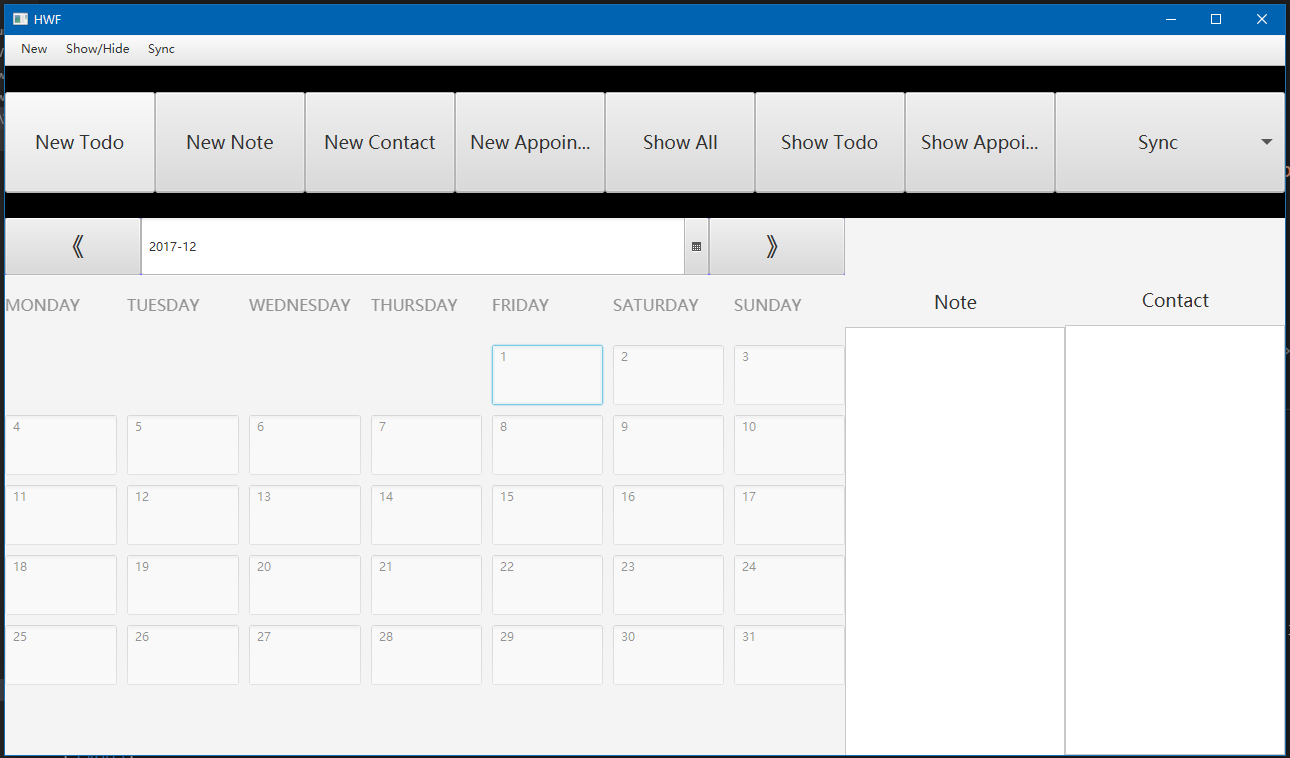
\includegraphics[width=10cm]{mainview.png}\\
        \end{figure}
    按下Create按钮创建新的PIMTodo项目并添加的数据模型的后台实现:
    \begin{lstlisting}[language=Java]
    public void Create(ActionEvent event){
        try{
            if(Contains.getText().length() == 0|| Priority.getText().length() == 0){
                throw new  Exception();
            }
            PIMTodo todo = new PIMTodo(Contains.getText(), LocalDate.parse(Year.getText()+Month.getText()+Day.getText(),DateTimeFormatter.ofPattern("yyyyMMdd")), Priority.getText());
            StarsRiver.MainWindows.pimcollection.add(todo);

            Stage stage = (Stage) Create.getScene().getWindow();
            Event.fireEvent(stage, new WindowEvent(stage, WindowEvent.WINDOW_CLOSE_REQUEST ));
        }
        catch(Exception e){
            Title.setText("Error");
        }
    }
    \end{lstlisting}

    从用户输入的域名和端口生成远程服务器的地址:
    \begin{lstlisting}[language=Java]
    public void Sync(ActionEvent event){
        try{
            if(HostName.getText().length() == 0|| Port.getText().length() == 0){
                //throw new  Exception();
            }
            StarsRiver.Controller.SyncNetWorkController.Url = HostName.getText() + ":" + Port.getText();
            StarsRiver.Controller.SyncNetWorkController.UrlReady = true;
            Stage stage = (Stage) Sync.getScene().getWindow();
            Event.fireEvent(stage, new WindowEvent(stage, WindowEvent.WINDOW_CLOSE_REQUEST ));
        }
        catch(Exception e){
            Title.setText("Error");
            StarsRiver.Controller.SyncNetWorkController.UrlReady = false;
        }
    }
    \end{lstlisting}


    按下NewTodo按钮,弹出NewTodo窗体
    \begin{lstlisting}[language=Java]
    public void NewTodo(ActionEvent event) throws Exception {
        Parent root = FXMLLoader.load(getClass().getResource("/View/NewTodo.fxml"));
        Stage primStage = new Stage();
        primStage.setTitle("New Todo");
        primStage.setScene(new Scene(root));
        primStage.show();
    }
    \end{lstlisting}


    打开文件选择器选择要同步的数据文件,同步数据并更新界面:
    \begin{lstlisting}[language=Java]
    public void SyncWithFile(ActionEvent event) {
        FileChooser fileChooser = new FileChooser();
        Stage primStage = new Stage();
        fileChooser.setTitle("Open PIMStore File");
        File file = fileChooser.showOpenDialog(primStage);
        if(file == null){
            return;
        }

        PIMStore store = new PIMFile();
        Sync(store, new String[]{file.getAbsolutePath()});
        updateView();
    }
    \end{lstlisting}

    与远程服务器同步数据并更新界面:
    \begin{lstlisting}[language=Java]
    public void SyncWithNetWork(ActionEvent event) throws Exception{
        Parent root = FXMLLoader.load(getClass().getResource("/View/SyncNetWork.fxml"));
        Stage primStage = new Stage();
        primStage.initModality(Modality.APPLICATION_MODAL);
        primStage.setOnCloseRequest(new EventHandler<WindowEvent>() {
            @Override
            public void handle(WindowEvent event) {
                if(SyncNetWorkController.UrlReady){
                    PIMStore store = new PIMNetwork();
                    Sync(store, new String[]{SyncNetWorkController.Url,"post"});
                    updateView();
                }
            }
        });
        primStage.setTitle("Input HostName and Port");
        primStage.setScene(new Scene(root));
        primStage.show();
    }
    \end{lstlisting}

    通过按钮调整视图模型中的date元素:
    \begin{lstlisting}[language=Java]
    public void DateBefor(ActionEvent event) {
        StarsRiver.MainWindows.date = StarsRiver.MainWindows.date.plusMonths(-1);
        updateView();
    }
    \end{lstlisting}

    设置界面中要呈现的数据类型
    \begin{lstlisting}[language=Java]
    public void ShowAll(ActionEvent event) {
        ShowTodo = !ShowTodo;
        ShowAppointment = !ShowAppointment;
        updateView();
    }
    \end{lstlisting}

    抽象出的数据同步过程,设置为先与向数据源追加写入当前视图模型中的数据,再从数据源读取全部数据并设置为视图模型中的数据。
    \begin{lstlisting}[language=Java]
    public static boolean Sync(PIMStore store,String[] str) {
        if(!store.Open(str)){
            System.out.println("Sync error");
            return false;
        }
        if(!store.Write(MainWindows.pimcollection.toStrings())){
            System.out.println("Sync error");
            return false;
        }
        store.Close();

        if(store.getClass()==PIMNetwork.class){
            str[1] = "all";
        }
        if(!store.Open(str)){
            System.out.println("Sync error");
            return false;
        }
        String[] data = store.Read();
        if(data == null){
            System.out.println("Sync error");
            return false;
        }
        store.Close();

        StarsRiver.MainWindows.pimcollection = new PIMCollection(data);
        return true;
    }
    \end{lstlisting}

    视图跟新过程,该过程应在视图模型数据变更后主动调用。
    \begin{lstlisting}[language=Java]
    private void updateView(){
        GridPane.clearConstraints(MainPane);
        MainPane.getChildren().removeAll(MainPane.getChildren());

        MainPane.setGridLinesVisible(true);
        MainPane.setOpacity(0.5);
        MainPane.setVgap(10);
        MainPane.setHgap(10);
        StringConverter converter = new StringConverter<LocalDate>() {
            DateTimeFormatter dateFormatter = 
                DateTimeFormatter.ofPattern("yyyy-MM");
            @Override
            public String toString(LocalDate date) {
                if (date != null) {
                    return dateFormatter.format(date);
                } else {
                    return "";
                }
            }
            @Override
            public LocalDate fromString(String string) {
                if (string != null && !string.isEmpty()) {
                    return LocalDate.parse(string, dateFormatter);
                } else {
                    return null;
                }
            }
        };  
        DateLab.setConverter(converter);
        DateLab.setValue(StarsRiver.MainWindows.date);

        for(int i = 0; i<7;i++){
            Label laber = new Label(DayOfWeek.of(i+1).toString());
            laber.setFont(new Font("Regular", 16));
            laber.setTextAlignment(TextAlignment.CENTER);
            MainPane.add(laber,i,0);
        }

        DateLab.setValue(MainWindows.date);

        LocalDate begin = MainWindows.date.with(TemporalAdjusters.firstDayOfMonth());
        LocalDate end = MainWindows.date.with(TemporalAdjusters.lastDayOfMonth());
        int beginDayOfWeek = begin.getDayOfWeek().getValue();
        int temp = 1;
        int dayOfMonth = 1;
        for(int j = 1; j < 7; j++){
            for(int i = 0; i < 7; i++){
                if(temp < beginDayOfWeek){
                    temp ++;
                    continue;
                }
                if(dayOfMonth <= end.getDayOfMonth()){
                    TextArea textArea = new TextArea();
                    textArea.setWrapText(true);
                    textArea.setFont(new Font("Regular", 12));

                    String str = Integer.toString(dayOfMonth) + "\n";
                    PIMCollection baseDate = StarsRiver.MainWindows.pimcollection.getItemsForDate(begin);
                    if(ShowTodo){
                        HashSet<PIMTodo> todos = baseDate.getTodos();
                        for (PIMTodo item : todos) {
                            str += item.toString() + "\n";
                        }
                    }
                    if(ShowAppointment){
                        HashSet<PIMAppointment> appointments = baseDate.getPIMAppointments();
                        for (PIMAppointment item : appointments) {
                            str += item.toString() + "\n";
                        }
                    }

                    textArea.setText(str);
                    textArea.setEditable(false);

                    MainPane.add(textArea,i,j);

                    begin = begin.plusDays(1);
                    dayOfMonth++;
                }
            }
        }
    \end{lstlisting}
\end{document}